\documentclass[border=2pt]{standalone}
\usepackage[T1]{fontenc}\usepackage{times}\usepackage{tikz}
\usetikzlibrary{positioning,arrows.meta,shapes.geometric}
\newcommand{\R}[1]{\textsf{R#1}}
\begin{document}
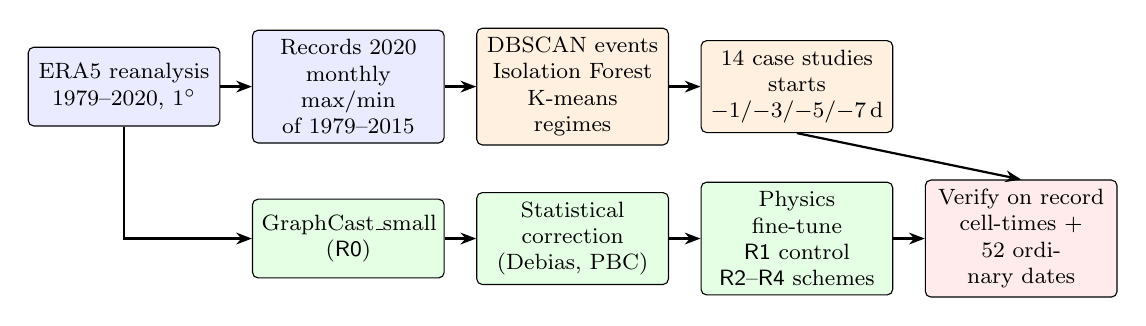
\begin{tikzpicture}[
  box/.style={draw, rounded corners=2pt, align=center, font=\footnotesize, minimum height=10mm, text width=22mm, fill=#1},
  box/.default=gray!8,
  arr/.style={-{Stealth[length=2mm]}, thick}]
\node[box=blue!8] (era) {ERA5 reanalysis\\1979--2020, 1$^\circ$};
\node[box=blue!8, right=4mm of era] (rec) {Records 2020\\monthly max/min\\of 1979--2015};
\node[box=orange!12, right=4mm of rec] (ml) {DBSCAN events\\Isolation Forest\\K-means regimes};
\node[box=orange!12, right=4mm of ml] (case) {14 case studies\\starts $-1/{-3}/{-5}/{-7}$\,d};
\node[box=green!10, below=7mm of rec] (r0) {GraphCast\_small\\(\R{0})};
\node[box=green!10, right=4mm of r0] (pbc) {Statistical\\correction\\(Debias, PBC)};
\node[box=green!10, right=4mm of pbc] (phys) {Physics fine-tune\\\R{1} control\\\R{2}--\R{4} schemes};
\node[box=red!8, right=4mm of phys] (ver) {Verify on record\\cell-times +\\52 ordinary dates};
\draw[arr] (era) -- (rec); \draw[arr] (rec) -- (ml); \draw[arr] (ml) -- (case);
\draw[arr] (era.south) |- (r0.west);
\draw[arr] (r0) -- (pbc); \draw[arr] (pbc) -- (phys); \draw[arr] (phys) -- (ver);
\draw[arr] (case.south) -- (ver.north);
\end{tikzpicture}
\end{document}
